% Präambel
% Angepasste Vorlage der DHBW Karlsruhe (http://zil.dhbw-karlsruhe.de/wiki/index.php/LaTeX/Vorlagen)
% Achtung: Ziemlich chaotisch, wird irgendwann mal aufgeräumt :-)

\documentclass[12pt,a4paper,oneside,
final, 
titlepage, 						% Titlepage-Umgebung statt \maketitle
headsepline, 					% horizontale Linie unter Kolumnentitel
%abstracton,					% Überschrift beim Abstract einschalten, Abstract muss dazu in{abstract}-Umgebung stehen 
%DIV11,							% auskommentieren, um den Seitenspiegel zu vergrößern
BCOR6mm,						% Bindekorrektur, die den Seitenspiegel um 6mm nach rechts verschiebt,
toc=listof,
parskip=full,
ngerman,
]{scrreprt}	
\usepackage{tabularx}		
\usepackage{ucs} 				% Dokument in utf8-Codierung schreiben und speichern
\usepackage[utf8x]{inputenc} 	% ermöglicht die direkte Eingabe von Umlauten
\usepackage[ngerman]{babel} 	% deutsche Trennungsregeln und Übersetzung der festcodierten Überschriften
\usepackage[T1]{fontenc} 		% Ausgabe aller zeichen in einer T1-Codierung (wichtig für die Ausgabe von Umlauten!)
\usepackage{graphicx}  			% Einbinden von Grafiken erlauben
\usepackage{amsmath}
%\usepackage{amsfonts}
%\usepackage{amssymb}
\usepackage[most]{tcolorbox}
\usepackage{mathpazo} 			% Einstellung der verwendeten Schriftarten
\usepackage{textcomp} 			% zum Einsatz von Eurozeichen u. a. Symbolen
\usepackage{xcolor} 			% einfache Verwendung von Farben in nahezu allen Farbmodellen
\usepackage{fancyhdr}			% Zusatzpaket zur Gestaltung von Fuß und Kopfzeilen
\usepackage[babel,german=quotes]{csquotes}
\usepackage{setspace}
\usepackage[all]{nowidow}
\usepackage{float}
\usepackage[format=plain,indention=0.5cm,hypcap=true]{caption}
\usepackage{paralist}
\usepackage{varioref}
\usepackage{hyperref}
\usepackage{translator}
\usepackage[toc,acronym]{glossaries} 	% zur Erstellung des Abkürzungsberzeichnisses
\usepackage{minted}
\usepackage[nameinlink]{cleveref}
\usepackage[nottoc]{tocbibind}
\usepackage[german,colorinlistoftodos]{todonotes}
\usepackage{pdfpages}

% spacing von matheumgebungen

\setlength{\jot}{10pt}

% Persönliche Daten:

\newcommand{\titel}{Titel der Arbeit}
\newcommand{\untertitel}{Untertitel der Arbeit}
\newcommand{\arbeit}{Typ der Arbeit (z.B. Praxisbericht)}
\newcommand{\studiengang}{Studiengang}
\newcommand{\autor}{Max Mustermann}
\newcommand{\matrikelnr}{007007}
\newcommand{\kurs}{Kursnummer}
\newcommand{\bearbeitungszeitraum}{01.01.2013 - 31.03.2013}
\newcommand{\firma}{Musterfirma GmbH, Karlsruhe}
\newcommand{\abgabe}{31. März 2013}
\newcommand{\betreuerdhbw}{Prof. Erika Mustermann}
\newcommand{\betreuer}{Markus Mustermann}

\newcommand{\jahr}{2013}

% Abkürzungen
\newcommand{\ua}{\mbox{u.\,a.\ }}
\newcommand{\zB}{\mbox{z.\,B.\ }}
\newcommand{\bs}{$\backslash$}
                       
% Eigenes Ref
\newcommand{\myref}[1]{vgl. \cref{#1} \nameref{#1} \vpageref{#1}}
\newcommand{\mylistingref}[1]{vgl. \cref{#1} \vpageref{#1}}

% Todogeschichten
\newcommand{\mytodo}[1]{\todo[color=red,inline]{#1}}
\newcommand{\mytodoimprove}[1]{\todo[color=green,inline]{#1}}

% inline code
\newcommand{\myinlinecode}[1]{\footnotesize\texttt{#1}\normalsize}

% Definition der Kopf- und Fußzeilen
\lhead{}								% Kopf links
\chead{}								% Kopf mitte
\rhead{\sffamily{\titel}}				% Kopf rechts
\lfoot{}								% Fuß links
\cfoot{\sffamily{\thepage}}				% Fuß mitte
\rfoot{\sffamily{\autor}}				% Fuß rechts
\renewcommand{\headrulewidth}{0.4pt}	% Liniendicke Kopf
\renewcommand{\footrulewidth}{0.4pt}	% Liniendicke Fuß

\makeglossaries							% Abkürzungsverzeichnis erstellen

% alle Abkürzungen, die in der Bachelorarbeit verwendet werden

\newacronym{DHBW}{DHBW}{Duale Hochschule Baden-Württemberg}
\newacronym{RHEL}{RHEL}{Red Hat Enterprise Linux}
\newacronym{CentOS}{CentOS}{Community Enterprise Operating System}
\newacronym{CPU}{CPU}{Central Processing Unit}
\newacronym{RAM}{RAM}{Random Access Memory}
\newacronym{HDD}{HDD}{Hard Disk Drive}
\newacronym{IIS}{IIS}{Internet Information Services}
\newacronym{TCP}{TCP}{Transmission Control Protocol}
\newacronym{UDP}{UDP}{User Datagram Protocol}
\newacronym{FIFO}{FIFO}{First In First Out}
\newacronym{AMQP}{AMQP}{Advanced Message Queueing Protocol}
\newacronym{GELF}{GELF}{Graylog Extended Logging Format}
\newacronym{REDIS}{redis}{Remote Dictionary Server}
\newacronym{API}{API}{Application Programming Interface}
\newacronym{JSON}{JSON}{JavaScript Object Notation}
\newacronym{HTML}{HTML}{Hypertext Markup Langauge}
\newacronym{JS}{JS}{JavaScript}
\newacronym{DHCP}{DHCP}{Dynamic Host Configuration Protocol}
\newacronym{EPEL}{EPEL}{Extra Packages for Enterprise Linux}
\newacronym{IP}{IP}{Internet Protocol}
\newacronym[longplural=virtuelle Maschinen]{VM}{VM}{virtuelle Maschine}
\newacronym{HTTP}{HTTP}{Hypertext Transfer Protocol}
\newacronym{URL}{URL}{Uniform Resource Locator}
\newacronym{SLA}{SLA}{Service Level Agreement}
\newacronym{CSV}{CSV}{Comma Separated Values}
\newacronym{ACID}{ACID}{Atomicity, Consistency, Isolation, Durability}
\newacronym[nonumberlist]{ZB}{z.B.}{zum Beispiel}
\newacronym[nonumberlist]{GGF}{ggf.}{gegebenenfalls}
\newacronym[nonumberlist]{ETC}{etc.}{et cetera (lat. für \textit{und die übrigen Dinge})}					% Datei mit Abkürzungen laden
%\newglossaryentry{Instrument}{
%	name=Instrument,
%	description={Begriff zur Umschreibung \ua folgender Sachverhalten im Bank- und Börsenwesen: Wertpapiere (\zB Aktien) oder Derivate}
%
					% Glossar laden

% Fix für minted, sodass unicode möglich ist
% http://tex.stackexchange.com/a/84883/15907

\makeatletter
\newcommand{\minted@write@detok}[1]{%
  \immediate\write\FV@OutFile{\detokenize{#1}}}%

\newcommand{\minted@FVB@VerbatimOut}[1]{%
  \@bsphack
  \begingroup
    \FV@UseKeyValues
    \FV@DefineWhiteSpace
    \def\FV@Space{\space}%
    \FV@DefineTabOut
    %\def\FV@ProcessLine{\immediate\write\FV@OutFile}% %Old, non-Unicode version
    \let\FV@ProcessLine\minted@write@detok %Patch for Unicode
    \immediate\openout\FV@OutFile #1\relax
    \let\FV@FontScanPrep\relax
%% DG/SR modification begin - May. 18, 1998 (to avoid problems with ligatures)
    \let\@noligs\relax
%% DG/SR modification end
    \FV@Scan}
    \let\FVB@VerbatimOut\minted@FVB@VerbatimOut

\renewcommand\minted@savecode[1]{
  \immediate\openout\minted@code\jobname.pyg
  \immediate\write\minted@code{\expandafter\detokenize\expandafter{#1}}%
  \immediate\closeout\minted@code}
\makeatother

% Minted Einstellungen %

\newminted[mycsharp]{csharp}{tabsize=2,fontsize=\footnotesize}
\newminted[mycsharplinenos]{csharp}{tabsize=2,xleftmargin=0.5cm,linenos,fontsize=\footnotesize}
\newminted[myjson]{js}{tabsize=2,fontsize=\footnotesize}
\newminted[myxml]{xml}{tabsize=2,fontsize=\footnotesize}
\newminted[myshell]{shell-session}{tabsize=2,fontsize=\footnotesize}
\newminted[mycode]{text}{tabsize=2,fontsize=\footnotesize}
\newminted[mycodelinenos]{text}{linenos,xleftmargin=0.5cm,tabsize=2,fontsize=\footnotesize}
\newminted[myruby]{ruby}{tabsize=2,fontsize=\footnotesize}
\renewcommand\listoflistingscaption{Codeverzeichnis}

% cref für minted listings
% http://tex.stackexchange.com/a/125029/15907

\makeatletter
\crefname{tcb@cnt@mintedbox}{Listing}{Listings}
\Crefname{tcb@cnt@mintedbox}{Listing}{Listings}
\makeatother

% % % % % % % % % % % % % % % % % % % % % % % % % % % % % % % % % % %
% % % Special Hack for getting minted to break lines
% http://tex.stackexchange.com/a/112573/15907

\usepackage{lineno}
\def\gobble#1{}
\renewcommand\DeleteFile[1]{}
\usepackage{xparse}
\ExplSyntaxOn
\box_new:N \l_fvrb_box
\tl_new:N \l_fvrb_tl

\RenewDocumentCommand \FancyVerbFormatLine { m }
 {
   \hbox_set:Nn \l_fvrb_box { #1 }
    \dim_compare:nNnTF { \box_wd:N \l_fvrb_box }>{ \linewidth }
      {%box to big 
       \tl_set:Nn \l_fvrb_tl { #1 }
       \fvrb_use_tl:N \l_fvrb_tl
      } 
      {%box fits
       \box_use:N \l_fvrb_box
      }
 }

\cs_new:Npn \fvrb_use_tl:N  #1
 {
  \group_begin:
   \null\hfill\vbox_set:Nn \l_fvrb_box
     {\hsize=\linewidth
      \renewcommand\thelinenumber
           {
             \ifnum\value{linenumber}=1\relax\else
                  $\rightarrow$
             \fi
           }
      \begin{internallinenumbers}
        \advance\hsize by -2em
        \hspace*{-2em}\tl_use:N #1
      \end{internallinenumbers}
     }
   \box_use:N \l_fvrb_box
  \group_end:
}

\ExplSyntaxOff

\usepackage{etoolbox}

% % % End of hack
% % % % % % % % % % % % % % % % % % % % % % % % % % % % % %

% Special listingsbox
% http://tex.stackexchange.com/a/124688/15907
\newenvironment{listingsbox}[3][]
 {%
   \def\listingsboxenvironment{#2}%save the environments
   \VerbatimEnvironment%
   \begin{mintedbox}[#1]{#3}%
     \begin{\listingsboxenvironment}}%
 {%
  \end{\listingsboxenvironment}%
  \end{mintedbox}%
}

\newtcolorbox[auto counter,
  list inside=mypyg]{mintedbox}[2][]{%
  title={Listing \thetcbcounter: #2},
  list entry={\numberline{\thetcbcounter}#2},
  enlarge right by={-0.5cm}, % no overfull hboxes for listing
  enhanced,breakable,#1}
  
% Mathe nur in Displaymode anzeigen
\everymath{\displaystyle}

% -------------------------------------------------------------------------------------------
%                     Beginn des Dokumenteninhalts
% -------------------------------------------------------------------------------------------
\begin{document}
\setcounter{secnumdepth}{3}					% Nummerierungstiefe für's Contentsverzeichnis
\setcounter{tocdepth}{2}					% Nummerierungstiefe für's Contentsverzeichnis
\sffamily									% für die Titelei serifenlose Schrift verwenden

% ------------------------------ Titelei -----------------------------------------------------

\thispagestyle{plain}
\begin{titlepage}
\enlargethispage{4.0cm}
\sffamily 								% Serifenlose Grundschrift für die Titelseite einstellen

\begin{minipage}[t][1.8cm][c]{0.481\textwidth}
\begin{flushleft}
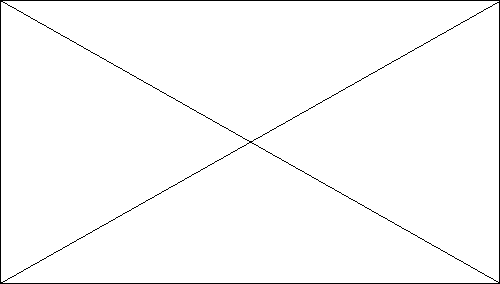
\includegraphics[width=6cm]{Images/placeholder.png}
\end{flushleft}
\end{minipage}
\begin{minipage}[t][1.8cm][c]{0.481\textwidth}
\begin{flushright}

\includegraphics[scale=2]{Images/logo_dhbw.jpg}
\end{flushright}
\end{minipage}
\\[5ex]
\begin{center}

\huge{\textsc{\textbf{\titel}}}\\[1ex]
\Large{\textbf{\untertitel}}\\[3ex]
\LARGE{\textbf{\arbeit}}\\[2ex]
\normalsize{für die Prüfung zum\\[1ex] Bachelor of Science}\\[3ex]
\Large{Studiengang \studiengang}\\[1ex]
\normalsize{Duale Hochschule Baden-Württemberg Karlsruhe}\\[5ex]
von\\[1ex] \autor \\[13ex]


\end{center}

\begin{flushleft}

\begin{tabular}{ll}
Abgabedatum:					& \quad \abgabe \\
Bearbeitungszeitraum:			& \quad \bearbeitungszeitraum   \\ 
Matrikelnummer, Kurs: 			& \quad \matrikelnr , \kurs \\ 
Ausbildungsfirma:	 			& \quad \firma \\ 
Betreuer der Ausbildungsfirma:  & \quad \betreuer \\
Gutachter der Dualen Hochschule: & \quad \betreuerdhbw \\ [5ex]

\end{tabular} 



\small
Copyrightvermerk:\\

Dieses Werk einschließlich seiner Teile ist \textbf{urheberrechtlich geschützt}. Jede Verwertung außerhalb der engen Grenzen des Urheberrechtgesetzes ist ohne Zustimmung des Autors unzulässig und strafbar. Das gilt insbesondere für Vervielfältigungen, Übersetzungen, Mikroverfilmungen sowie die Einspeicherung und Verarbeitung in elektronischen Systemen.
\end{flushleft}
\begin{flushright}
\copyright{} \jahr
\end{flushright}
\end{titlepage} 				% erzeugt die Titelseite
\pagenumbering{Roman}						% große, römische Seitenzahlen für Titelei
% Sperrvermerk bei Bedarf dekommentieren
\addchap*{Sperrvermerk}
\normalsize

Die vorliegende Arbeit beinhaltet interne vertrauliche Informationen der Firma
\firma. Die Weitergabe des Inhalts der Arbeit im Gesamten oder in
Teilen sowie das Anfertigen von Kopien oder Abschriften - auch in digitaler Form
- sind grundsätzlich untersagt. Ausnahmen bedürfen der schriftlichen Genehmigung
der Firma \firma sowie des Autors \autor.

\pagebreak

\addchap*{Eidesstattliche Erklärung}
Ich versichere hiermit, dass ich meinen Praxisbericht mit dem Thema
\begin{quote}
\textit{\titel\ - \untertitel}
\end{quote}
selbständig verfasst und keine anderen als die angegebenen Quellen und Hilfsmittel benutzt habe. Die Arbeit wurde bisher keiner anderen Prüfungsbehörde vorgelegt und auch nicht veröffentlicht.\\[10ex]

Karlsruhe, den \today \\[4ex]


\rule[-0.2cm]{5cm}{0.5pt} \\

\textsc{\autor} \\[10ex] 				% Einbinden der eidestattlichen Erklärung

\addchap*{Abstract / Zusammenfassung}


\tableofcontents							% Erzeugen des Inhalsverzeichnisses
\deftranslation[to=German]{Acronyms}{Abk\"urzungsverzeichnis}
\glsaddall[types={acronym}]					% Alle Akronyme ausgeben
\printglossary[type=\acronymtype]						% Erzeugen des Abkürzungsverzeichnisses
\listoffigures 								% Erzeugen des Abbildungsverzeichnisses 
\listoftables 								% Erzeugen des Tabellenverzeichnisses
\tcblistof[\addchap*]{mypyg}{Codeverzeichnis} % Erzeugen eines Verzeichnisses für Code
\addcontentsline{toc}{chapter}{Codeverzeichnis}
\todototoc
\listoftodos
\clearpage

% --------------------------------------------------------------------------------------------
%                    Content der Bachelorarbeit
%---------------------------------------------------------------------------------------------
\pagenumbering{arabic}						% arabische Seitenzahlen für den Hauptteil
\pagestyle{fancy}					
\rmfamily
\onehalfspacing
% Schusterjungen und Hurenkinder 
%\clubpenalty = 10000
%\widowpenalty = 10000 \displaywidowpenalty = 10000
\interfootnotelinepenalty=10000 % Keine FUßnoten umbrechen
\chapter{Einleitung}

\section{Problematik}

\section{Ziel}

\section{Abgrenzung}
\clearpage
\chapter{Grundlagen}

\clearpage
\chapter{Konzept}
\clearpage
\chapter{Implementierung}

\section{ToDo}

Um ToDos anzuzeigen können alle Befehle des Packages \enquote{todonotes}\footnote{\url{http://www.ctan.org/tex-archive/macros/latex/contrib/todonotes/}} genutzt werden.
Zur Einfachheit können folgende Befehle genutzt werden:

\begin{verbatim}
\mytodo{Kapitel über Krokodile schreiben!}
\mytodoimprove{Neue Quellen raussuchen!}
\end{verbatim}

\mytodo{Kapitel über Krokodile schreiben!}
\mytodoimprove{Neue Quellen raussuchen!}

\section{Literaturverzeichnis}

Das Literaturverzeichnis generiert die Einträge nach DIN 1502-2. Die Styles sind in der alphadin.bst\footnote{\url{http://mirror.unl.edu/ctan/biblio/bibtex/contrib/german/din1505/alphadin.bst}} zu finden.

Beispiele \cite{web:wiki:latex,book:komascript}

\section{Verzeichnisse}

Dieses Template erstellt einige Verzeichnisse, wie sie entsprechend der DHBW-Richtlinien benötigt werden: Inhaltsverzeichnis, Abbildungsverzeichnis, Tabellenverzeichnis, Abkürzungsverzeichnis und Codeverzeichnis

Zur Demonstration einige Beispiele:

\begin{figure}[H]
\centering
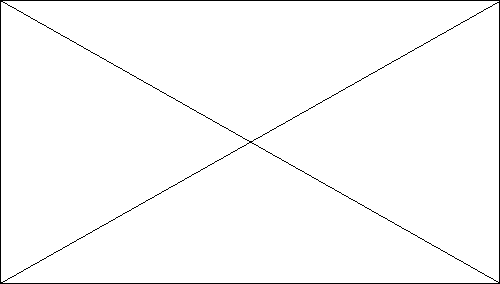
\includegraphics[width=\textwidth]{Images/placeholder.png}
\caption{Ich bin ein tolles Bild!}
\end{figure}

\begin{table}[H]
\centering
\begin{tabular}{ll}
	\textbf{Kopfspalte 1} & \textbf{Kopfspalte 2} \\ \hline\hline
	Ich bin               & eine tolle Tabelle!   \\ \hline
	Bin ich               & nicht wundervoll?
\end{tabular}
\caption{Eine tolle Tabelle}
\end{table}

\section{Source code}

Gerade im IT-Bereich kommt es oft vor, dass Source eingebunden werden soll. Natürlich schön mit Syntax-Highlighting. 
Dieses Template unterstütz dies mit Hilfe von minted\footnote{\url{http://www.ctan.org/tex-archive/macros/latex/contrib/minted/}} und pygments\footnote{\url{http://pygments.org/}}. Die Einrichtung dafür ist beschrieben unter \url{http://www.manuel-rauber.com/post/2013/10/28/My-LaTeX-Environment}.
Des Weiteren ist das Template in der Lage, lange Zeilen umzubrechen\footnote{Allerdings hat die Funktion noch einen Bug: \url{http://tex.stackexchange.com/questions/129383/break-lines-in-minted-code}. Bei bereits eingerücktem Code werden die \enquote{Umbruchpfeile} falsch dargestellt.}, sowie Captions und Boxen anzuzeigen. Zu lange Code-Stücke werden automatisch auf die nächste Seite umgebrochen, was man auch visuell sehen kann. Hier für ein längeres Code-Beispiel:

\begin{listingsbox}{mycsharplinenos}{Beispiel-Code}
using System;
using System.IO;
using System.Net;
using System.Net.Http;
using System.Net.Http.Formatting;
using System.Net.Http.Headers;
using System.Text;
using System.Threading.Tasks;

namespace ShortUrl.Core.Formatters
{
	public class TextMediaTypeFormatter : MediaTypeFormatter
	{
		public TextMediaTypeFormatter()
		{
			SupportedEncodings.Add(Encoding.UTF8);
		}

		public override Task WriteToStreamAsync(Type type, object value, Stream writeStream, HttpContent content,
			TransportContext transportContext)
		{
			return Task.Factory.StartNew(() =>
			{

				var str = (string)value;

				using (var textWriter = new StreamWriter(writeStream))
				{
					textWriter.Write(str);
				}
			});
		}

		public override bool CanReadType(Type type)
		{
			return false;
		}

		public override bool CanWriteType(Type type)
		{
			return typeof(string) == type;
		}
	}
}
\end{listingsbox}

\section{Glossar}

Der Aufbau eines Glossar wird entsprechend durch das Package \enquote{glossaries}\footnote{\url{http://www.ctan.org/tex-archive/macros/latex/contrib/glossaries/}} unterstützt.

Du wolltest schon immer mal wissen, was ein \gls{Instrument} ist? ;-)

\clearpage
\chapter{Ergebnis}

% ------------------------------- Anhang ---------------------------------------------------------

\appendix
\clearpage
\pagenumbering{Roman}						% römische Seitenzahlen für Anhang

% Bibliographie nach DIN 1502-2
\bibliographystyle{alphadin} 
\bibliography{Bibliography}
\clearpage
\printglossary
\end{document}